\vspace{2mm}
\section{DLO-Lab Benchmark}
Built upon the differentiable simulator, our DLO-Lab benchmark provides a versatile collection of DLO manipulation tasks equipped with differentiable reward functions. 
We also offer standardized APIs for building new manipulation environments.
Our proposed tasks are illustrated in~\Cref{fig:tasks}. 

\subsection{Benchmark Representation}
\textbf{Task Formulation}
We address a series of manipulation tasks where an agent uses a set of robot arms equipped with parallel grippers to achieve specific goals.
We formulate each task as a standard finite-horizon Markov Decision Process (MDP). Specifically, an MDP is comprised of a state space $\gS$, an action space $\gA$, a transition function $\gT: \gS \times \gA \rightarrow \gS$, and a reward function associated with each transition step $\gR: \gS \times \gA\times \gS \rightarrow \sR$. We optimize the agent to derive a policy $\pi(a|s)$ that maximizes the expected sum of discounted rewards, $E_\pi \big[\sum_{t=0}^T \gamma^t \gR (s_t, a_t)\big]$, over a horizon $T$ with a discount factor $\gamma$.

\textbf{State Space}
Let $\text{N}_v$ denote the total number of vertices of all DLOs in the scene, and let $\text{N}_m$ denote the total degrees of freedom (DoF) for all robot arms. The complete simulation state for the system is represented as:
$
\rmS = (\rvx, \dot{\rvx}, \rvr, \rmM, \dot{\rmM}),
$
where $\rvx, \dot{\rvx} \in \mathbb{R}^{\text{N}_v \times 3}$ gives the positions and velocities of all DLO vertices, $\rvr \in \mathbb{R}^{\text{N}_v\times 3}$ encodes the rest configurations, and $\rmM, \dot{\rmM} \in \mathbb{R}^{\text{N}_m}$ denote the joint positions and velocities of the robot arms.

\begin{figure*}[t]
    \begin{center}
        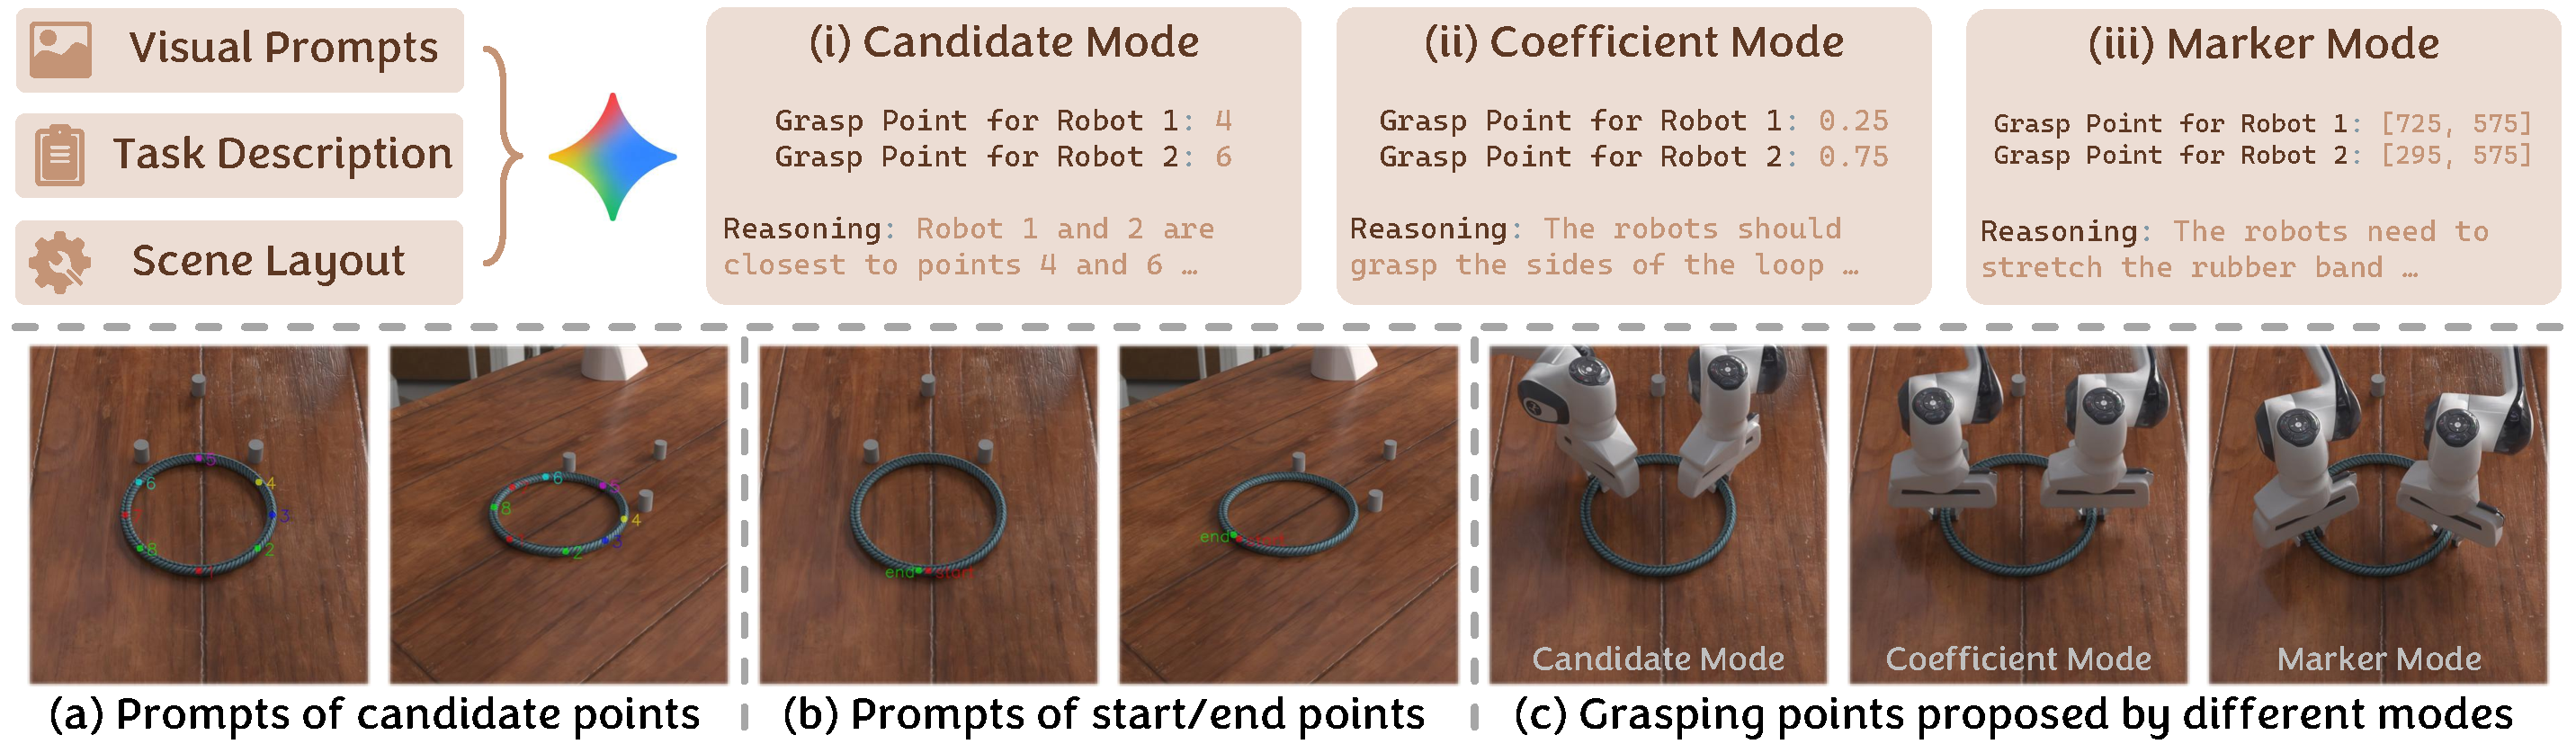
\includegraphics[width=\linewidth]{figs/agent_point_v3.pdf}
    \end{center}
    \vspace{-4mm}
    \caption{
        \textbf{DLO agent for grasping point proposal.} To decide the grasping points for robust DLO manipulation, we feed the DLO agent with task-related information and design three output modes, each with a different modality. We observe that \textit{Candidate} mode yields the best reliability in our preliminary experiments (see Appendix~\ref{sec:comparison_grasp_proposal}) and thus adopt it by default.
    }
    \label{fig:agent_grasping_proposal}
\vspace{-4mm}
\end{figure*}

\textbf{Observation}
Unlike other deformable-material manipulation settings~\citep{huangplasticinelab,xianfluidlab,hoang2025geometryaware} where downsampling is required to reduce the dimensionality of the observation space, in our case, it is computationally feasible to leverage the full state of the DLOs. Thus, the observation space for the DLOs consists of the stacked positions and velocities $(\rvx, \dot{\rvx})$, resulting in an $\text{N}_v \times 6$ representation. To capture the robot side of the interaction, we augment the observation with each manipulator’s end-effector position $\rvp^\text{ef}_i$ and orientation $\rvo^\text{ef}_i$, along with the current joint configuration $\rmM$. When additional objects are presented, we also include the center-of-mass position and velocity of each object. This yields a complete observation vector that provides the agent with direct access to both the DLO dynamics and the manipulator kinematics, ensuring sufficient information for closed-loop control.

\textbf{Action Space}  
We implement end-effector pose control for the robot arms. At each step, the action specifies the gripper's target pose in Cartesian space. An inverse kinematics (IK) solver~\citep{pink} is then used to determine the joint configurations required to reach these targets. This approach enables the policy to operate directly in task space, simplifying the robot's kinematics and ensuring the precise spatial alignment required for DLO manipulation.

\subsection{Manipulation Tasks}
\label{sec:manipulation_tasks}

\begin{figure*}[t]
    \begin{center}
        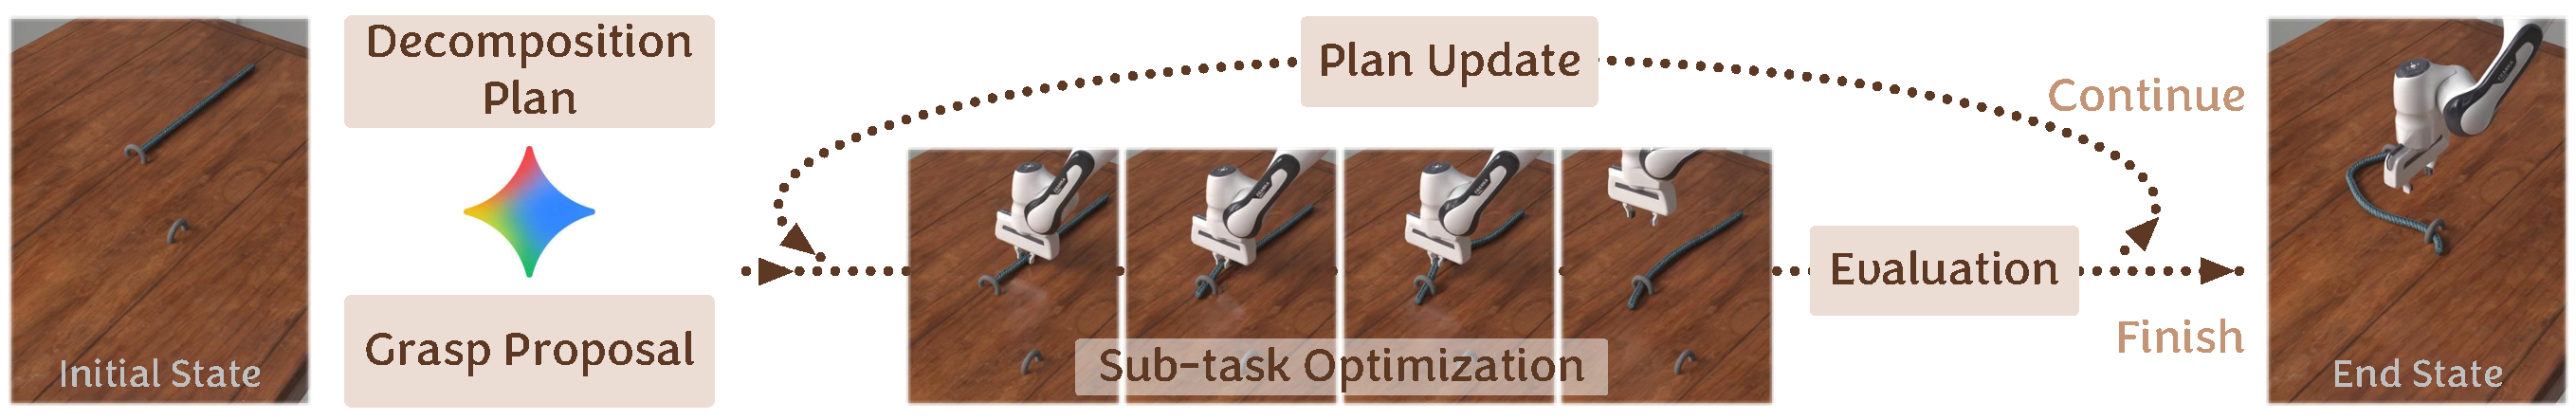
\includegraphics[width=\linewidth]{figs/agent_task_v1.pdf}
    \end{center}
\vspace{-2mm}
    \caption{
        \textbf{DLO agent for task decomposition.} The DLO agent begins by proposing an initial task decomposition plan based on the need to change grasping points. We then perform iterative trajectory optimizations and provide the resulting trajectories to the agent for evaluation. It will continually update the sub-task plan and execute the next sub-task optimization until the task is deemed complete.
    }
    \label{fig:agent_task_decomposition}
\end{figure*}

\textbf{Coiling}\quad The scene consists of a fixed cone and a rope. The agent needs to wind the rope around the cone's surface.
\vspace{-1mm}

\textbf{Gathering}\quad This task starts with several rigid and deformable bodies randomly placed on the ground. The objective is to use a rope to gather these objects together.
\vspace{-1mm}

\textbf{Lifting}\quad Given two ``C''-shaped rings, the agent is required to manipulate a rope to lift the rings.
\vspace{-1mm}

\textbf{Separation}\quad In this task, the agent needs to use two robot arms to separate two ropes that are initially tangled together.
\vspace{-5mm}

\textbf{Slingshot}\quad In this scenario, a rigid ball and a rigid cube are placed on a table. In front of the ball, there is a slingshot made from a rope with high stretching stiffness. The agent should operate a robot arm and use the slingshot to launch the ball and hit the cube.
\vspace{-1mm}

\textbf{Unknotting}\quad This task requires the agent to untangle a rope that has an overhand knot.
\vspace{-1mm}

\textbf{Wiring-post}\quad The task involves manipulating a rope from a straight position into a specific ``S''-shaped path that winds through two posts fixed to the table.
\vspace{-1mm}

\textbf{Wrapping}\quad The agent is asked to wrap a rubber band around three cylinders fixed to the table.
\vspace{-1mm}

\textbf{Letter Art}\quad The scene begins with three straight ropes, a fixed rubber band, and three posts fixed to the table. The agent should bend the three straight ropes to form the letters ``D'' and ``L''. When combined with the rubber band, the final arrangement should display ``DLO''.
\vspace{-1mm}

\textbf{Wiring-ring}\quad In this task, the agent needs to wire a rope through two rings fixed to the table.

Please see Appendix~\ref{sec:task_setup}-\ref{sec:reward_design} for additional details on task setups. We also relate the designed tasks to real-world manipulation skills in Appendix~\ref{sec:real_world_mapping}.



\subsection{DLO Agent}
\label{sec:agent}

In DLO manipulation, the challenges of co-dimensional properties and underactuated dynamics can make it hard for end-to-end policies to effectively explore the action space, especially in long-horizon tasks with complex topologies. To tackle these issues, we present a specialized DLO agent integrating structural priors into the manipulation process.

\textbf{Grasp Proposal} The selection of grasping points is a critical determinant of success in DLO manipulation. In tasks such as \textit{Unknotting}, selecting a suboptimal grasp can render the objective kinematically unsolvable. While manual specification of contact points is tedious and inefficient, random sampling is computationally prohibitive due to the vast search space. To address this, we leverage a Vision-Language Model (VLM) to propose grasping points guided by physical commonsense. As illustrated in~\Cref{fig:agent_grasping_proposal}(d), we design three distinct prompting modes for this capability:
(1) \textit{Candidate} mode: The system uniformly samples points along the DLO, as in~\Cref{fig:agent_grasping_proposal}(a), and queries the VLM to select the optimal candidate.
(2) \textit{Coefficient} mode: The VLM is provided with the DLO's endpoints, as in~\Cref{fig:agent_grasping_proposal}(b), and prompted to output a scalar coefficient in $[0, 1]$, representing the normalized position of the grasp along the DLO's length.
(3) \textit{Marker} mode: The VLM is given visual markers for the DLO's endpoints, as in~\Cref{fig:agent_grasping_proposal}(b), and is tasked with directly pinpointing the pixel coordinates of the suitable grasp on the rendered image.
We evaluate these approaches in Appendix~\ref{sec:comparison_grasp_proposal} and find that \textit{Candidate} mode consistently yields superior reliability and leads to better results. Thus, we adopt this mode for our subsequent experiments.

\begin{table*}[t]
\centering
\scalebox{0.9}{
\setlength{\tabcolsep}{1.2mm}{
\begin{tabular}{l|cccccccc}
    \toprule
    \bf Tasks  & \bf Coiling & \bf Gathering & \bf Lifting & \bf Separation & \bf Slingshot & \bf Unknotting & \bf Wiring-post & \bf Wrapping  \\
    \midrule
    \bf PPO      & 9.40$\pm$0.07 & 39.76$\pm$0.12 & 247.38$\pm$0.20 & 114.31$\pm$13.21 & 6.90$\pm$0.00 & 3.29$\pm$0.00 & 62.17$\pm$1.97 & 131.08$\pm$7.20 \\
    \bf SAC      & 8.28$\pm$0.74 & 40.76$\pm$0.53 & 250.29$\pm$2.44 & \bf 134.71$\pm$0.93 & 7.23$\pm$0.23 & 2.95$\pm$0.03 & 62.07$\pm$0.73 & 161.85$\pm$1.59 \\
    \midrule
    \bf SHAC     & 11.55$\pm$0.15 & 40.48$\pm$0.51 & 214.24$\pm$23.87 & 96.29$\pm$20.53 & 6.90$\pm$0.00 & 45.88$\pm$0.12 & 36.42$\pm$3.91 & 129.90$\pm$16.06 \\
    \bf SAPO     & 11.57$\pm$0.07 & 40.29$\pm$0.33  & 204.54$\pm$18.70 & 105.27$\pm$14.87 & 6.90$\pm$0.00 & 46.30$\pm$0.49 & 36.13$\pm$2.83 & 144.36$\pm$8.18 \\
    \midrule
    \bf GD       & 11.59 & 39.84 & 255.55 & 115.52 & 6.90 & 3.44 & 36.40 & 139.98 \\
    \bf CMA-ES   & \bf 11.73$\pm$0.02 & \bf 47.84$\pm$0.35 & \bf 335.59$\pm$14.21 & 84.86$\pm$0.40 & \bf 11.07$\pm$0.43 & \bf 57.21$\pm$1.51 & \bf 64.31$\pm$0.56 & \bf 162.68$\pm$0.86 \\
    \bottomrule
\end{tabular}
}}
\caption{\textbf{DLO-Lab tasks tabular results.} We show the maximum episodic return within a fixed number of episodes and its standard deviation for the 8 fixed-horizon tasks over 3 random seeds. Since GD has no randomness in different trials, it has no standard deviation.}
    \label{tab:quantitative}
\vspace{-6mm}
\end{table*}

\textbf{Task Decomposition} Beyond the spatial challenge of grasping, the complexity of DLO manipulation is further compounded by the sequential dependencies inherent in long-horizon tasks. In these scenarios, a single continuous motion is often insufficient; the robot must strategically re-grasp the object and adapt to intermediate deformations. Consequently, standard end-to-end policy learning often struggles with the exploration problem, as fixed reward functions fail to effectively guide the agent through the extensive combinatorial space of possible actions. To mitigate this, we employ agentic task decomposition. As depicted in~\Cref{fig:agent_task_decomposition}, the process begins by prompting the VLM to generate an initial decomposition plan based on the task description. This plan explicitly defines the reward function and horizon length for each sub-task, along with the criteria for final success. Utilizing the grasp proposal, we then optimize each sub-task sequentially.
A crucial step in this process is the closed-loop evaluation: after each execution, we render the optimized trajectory and ask the agent to assess whether the task has been completed. If the objective has not yet been achieved, the agent dynamically updates the plan for later phases based on the current state, ensuring the policy remains robust to execution errors. We evaluate the proposed agentic task decomposition on the two long-horizon tasks and present the results in Appendix~\ref{sec:analysis_task_decomposition}. 